\chapter{Methodology and System Design}
\label{cha:methodology_sys_design}


\section{The INVEKOS Dataset}
\label{sec:invek_dataset}

To evaluate the proposed sequence-modeling architectures, experiments were conducted using the Austrian INVEKOS (Integrated Administration and Control System) dataset.
INVEKOS serves as the European Union's official spatial registry for agricultural parcel identification, providing rich,
multi-year ground-truth vector data based on farmers' declarations \cite{perantoni_bayesian_2024}. 

It is important to explicitly state that the data extraction and pre-processing pipeline utilized in this thesis was originally designed and
implemented by Perantoni et al. \cite{perantoni_bayesian_2024}. By adopting their highly optimized dataset structure,
this research was able to bypass standard preprocessing bottlenecks and focus entirely on the architectural development of neural network sequence models. 

For this project, the spatial boundaries and crop labels were matched with Sentinel-2 Level-1C (L1C) optical imagery,
specifically focusing on the Military Grid Reference System (MGRS) tile 33UVP \cite{perantoni_bayesian_2024}.
This provided a continuous, six-year acquisition period spanning from September 2016 to September 2022,
encompassing a total of 805 satellite acquisitions with all 13 spectral channels resampled to a 10m resolution \cite{perantoni_bayesian_2024}.

\begin{table}[htpb]
    \centering
    \renewcommand{\arraystretch}{1.2}
    \begin{tabular}{ll}
        \toprule
        \textbf{Parameter} & \textbf{Value} \\
        \midrule
        Data Source & Sentinel-2 L1C \& INVEKOS \\
        Tile & MGRS 33UVP \\
        Timeframe & Sept 2016 -- Sept 2022 \\
        Total Acquisitions & 805 \\
        Spatial Resolution & 10m \\
        Number of Classes & 47 \\
        Minimum Parcel Area & 400 m$^2$ \\
        Erosion Buffer & 15m \\
        Data Splits & 60\% Train, 20\% Val, 20\% Test \\
        \bottomrule
    \end{tabular}
    \caption{Summary of the INVEKOS dataset and extraction parameters.}
    \label{tab:dataset_params}
\end{table}

\subsection{Data Acquisition (Spatial Patches vs. 1D Pixel Data)}
\label{subsec:data_acquisition}

A critical challenge in pixel-based crop mapping is the presence of "mixed pixels" at the boundaries of agricultural parcels,
which contain overlapping spectral signatures from neighboring fields. To mitigate this, a stringent geometric preprocessing pipeline
was applied to the INVEKOS shapefiles \cite{perantoni_bayesian_2024}. 

Instead of extracting raw 2D spatial patches, spatial erosion buffers were applied to the interior of all field polygons to exclude border pixels.
Furthermore, a minimum area threshold of 400 m$^2$ was enforced to ensure only sufficiently large and homogeneous parcels were retained \cite{perantoni_bayesian_2024}.
The refined, eroded geometries were subsequently rasterized to align precisely with the Sentinel-2 pixel grid. Finally, to optimize memory overhead,
each crop field was collapsed into a single 1D entry representing the spatial mean value of the pixels belonging to that field on every acquisition date \cite{perantoni_bayesian_2024}.
This filtering process yielded an exceptionally clean dataset containing 47 distinct crop type labels \cite{perantoni_bayesian_2024}.

\subsection{Pre-processing and Handling Irregular Time Series}
\label{subsec:preprocessing}

Handling massive spatial-temporal raster datasets alongside dense vector geometries introduces severe I/O bottlenecks in standard machine learning pipelines.
To overcome this, the 1D Sentinel-2 time series data and corresponding ground-truth representations were converted into a streamlined HDF5 (\texttt{.h5}) format,
and subsequently into a Lightning Memory-Mapped Database (LMDB) format.

This database architecture enables fast, memory-mapped data reading without requiring the entire multi-gigabyte dataset to be loaded into system RAM.
As implemented through the project's PyTorch Lightning \texttt{InvekosDataModule}, the dataset enforces a rigorous stratified random sampling partitioning strategy
to ensure unbiased evaluation \cite{perantoni_bayesian_2024}. The data is split using a standard ratio of 60\% for training, 20\% for validation,
and 20\% for testing \cite{perantoni_bayesian_2024}. This optimized 1D data structure feeds perfectly into data loaders configured with multi-worker pre-fetching,
ensuring high throughput across High-Performance Computing (HPC) nodes.

\section{Single-Year Non-Hybrid Baselines}
\label{subsec:single_year_baselines}

To establish a rigorous benchmark for multi-year architectures, two single-year sequence modeling baselines were developed and evaluated.
These models process intra-year phenological data to provide a comparative standard against which the complexity of hybrid and multi-year models can be justified.

\subsection{Temporal 1D Convolutional Neural Network (CNN)}
The first baseline is a 1-Dimensional Convolutional Neural Network (1D-CNN) designed to extract temporal features by sliding convolutional
filters across the time dimension, a methodology that has proven highly effective for satellite time series classification \cite{pelletier_temporal_2019}.
The \textbf{encoder} consists of two sequential convolutional blocks.
The initial layer maps the 13 input satellite bands to 64 channels using a kernel size of 3 and a padding of 1 to preserve the temporal sequence length.
This is followed by a 1D Batch Normalization layer and an in-place ReLU activation to introduce non-linearity.
The second layer further projects the features from 64 to 128 channels, utilizing the same kernel size, padding, normalization, and activation parameters.
For \textbf{classification}, a point-wise convolution (kernel size of 1) is applied to map the extracted 128-dimensional features to the 47 crop classes.
To generate the final field-level classification, the network executes a temporal majority vote by averaging the logit predictions across all time steps in the year.

\begin{figure}[htpb]
    \centering
    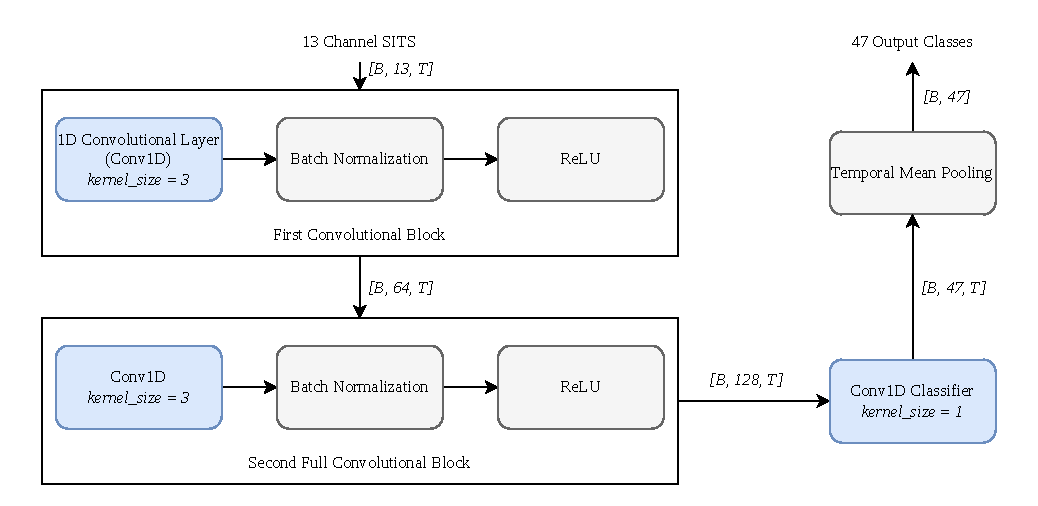
\includegraphics[width=0.8\textwidth]{images/cnn_diagram.pdf}
    \caption{Architectural block diagram of the Temporal 1D-CNN baseline.}
    \label{fig:cnn_architecture}
\end{figure}

\subsection{Temporal Gated Recurrent Unit (GRU RNN)}
The second baseline leverages a Gated Recurrent Unit (GRU) \cite{cho_learning_2014} to explicitly model the sequential dependencies of agricultural phenology.
A \textbf{bidirectional GRU} architecture is utilized to process the temporal sequences in both forward and backward directions,
yielding better performance than a standard unidirectional RNN. The input tensors are systematically permuted to align the time and channel dimensions for batch-first sequence processing.
Instead of averaging predictions over time, the network isolates the final temporal output step.
This final hidden state is fed into a fully connected linear \textbf{classifier} to predict the 47 crop classes.
Because the network is bidirectional, the input dimension of the final linear classifier is explicitly doubled to accommodate the concatenated forward and backward hidden features.
To assess the optimal architectural capacity, the hyperparameter search space tests varying hidden dimensions (128, 256, and 512) and depth configurations (1, 2, and 3 stacked layers).

\begin{figure}[htpb]
    \centering
    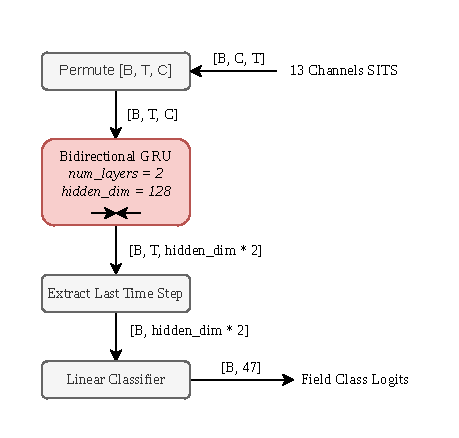
\includegraphics[width=0.8\textwidth]{images/gru_diagram.pdf}
    \caption{Architectural diagram of the Bidirectional GRU baseline.}
    \label{fig:gru_architecture}
\end{figure}


\section{Multi-Year Hybrid Architecture}
\label{sec:hybrid_architecture}

The core contribution of this thesis is the development of a hybrid, multi-scale neural architecture capable of simultaneously modeling intra-year
phenological dynamics and inter-year crop rotation patterns. Unlike traditional approaches that treat multi-year classification as independent yearly tasks,
this architecture hierarchically processes continuous, multi-year sequences end-to-end. 

\subsection{AgroDays Positional Encoding}
\label{subsec:agrodays_encoding}

The first step in the data pipeline is preparing the raw inputs for sequence modeling.
The raw 1D pixel sequence, consisting of 13 spectral channels, is initially projected into a higher-dimensional embedding space (128 dimensions).
However, standard sequence models assume that data points arrive at regular, evenly spaced intervals.
Agricultural satellite time series are inherently irregularly sampled due to cloud cover and varying satellite revisit times.
Using standard sequential positional encodings would falsely inform the model that all observations are equidistant.
To address this, the architecture utilizes a custom \textbf{AgroDays Positional Encoding} module.
Instead of simply indexing observations as sequential integer steps, this module adapts the standard sinusoidal positional
encoding \cite{attention_is_all_you_need} by scaling the frequencies using the exact agricultural day of the acquisition.
By calculating the encoding angles based on the absolute temporal position of the specific acquisition day, the model inherently understands the varying,
irregular time gaps between observations, ensuring the network accurately aligns the spectral data with the correct stage of the crop's phenological cycle.

\begin{algorithm}[htpb]
    \caption{AgroDays Positional Encoding}
    \label{alg:agrodays}
    \begin{algorithmic}[1]
        \Require Flattened input sequence $X \in \mathbb{R}^{(B \cdot Y) \times T \times d\_model}$
        \Require Agricultural days matrix $pos \in \mathbb{R}^{(B \cdot Y) \times T}$
        \Ensure Position-encoded sequence $X_{enc} \in \mathbb{R}^{(B \cdot Y) \times T \times d\_model}$
        \vspace{1.5mm}
        \State $div\_term \gets \exp\left(\text{arange}(0, d\_model, 2) \cdot \frac{-\ln(10000.0)}{d\_model}\right)$
        \State $pos\_expanded \gets \text{unsqueeze}(pos, \text{dim}=-1)$
        \State $angles \gets pos\_expanded \times div\_term$
        \State $PE \gets \text{zeros\_like}(X)$
        \State $PE_{:,:,0::2} \gets \sin(angles)$ \Comment{Apply sine to even indices}
        \State $PE_{:,:,1::2} \gets \cos(angles)$ \Comment{Apply cosine to odd indices}
        \State $X_{enc} \gets X + PE$ \Comment{Inject temporal signal into embeddings}
        \State \textbf{return} $X_{enc}$
    \end{algorithmic}
\end{algorithm}

\subsection{The Hierarchical Transformer-LSTM Model}
\label{subsec:transformer_lstm}

Once the position-aware embeddings are generated, the network processes the temporal scales using a two-stage hierarchical model. 
In the first stage, the objective is to understand the intra-year phenological growth cycle.
To optimize computational efficiency, the multi-year input tensor is reshaped, flattening the batch and year dimensions together.
This allows an Intra-Year Transformer Encoder to process every year independently and in parallel across the GPUs.
Driven by Multi-Head Self-Attention \cite{attention_is_all_you_need}, the Transformer evaluates the entire yearly sequence simultaneously,
effectively capturing complex growth stages without being hindered by vanishing gradients \cite{russwurm_self_attention_2020}.

\begin{algorithm}[htpb]
    \caption{Hierarchical Transformer-LSTM Forward Pass}
    \label{alg:hybrid_forward}
    \begin{algorithmic}[1]
        \Require Multi-year input tensor $X \in \mathbb{R}^{B \times Y \times C \times T}$
        \Require Agricultural days tensor $pos \in \mathbb{R}^{B \times Y \times T}$
        \Ensure Crop class logits $Y_{pred} \in \mathbb{R}^{B \times n\_classes \times Y}$
        \vspace{1.5mm}
        \State \textbf{Stage 1: Intra-Year Processing (Transformer)}
        \State $X \gets \text{permute}(X, [0, 1, 3, 2])$ \Comment{Target shape: $[B, Y, T, C]$}
        \State $X_{flat} \gets \text{reshape}(X, [B \cdot Y, T, C])$ \Comment{Flatten for independent yearly processing}
        \State $pos_{flat} \gets \text{reshape}(pos, [B \cdot Y, T])$
        \State $X_{emb} \gets \text{LinearProjection}(X_{flat})$
        \State $X_{emb} \gets \text{AgroDaysPositionalEncoding}(X_{emb}, pos_{flat})$
        \State $T_{out} \gets \text{TransformerEncoder}(X_{emb})$ \Comment{Self-Attention over time steps}
        \State $Y_{emb} \gets \text{mean}(T_{out}, \text{dim}=1)$ \Comment{Temporal pooling: $[B \cdot Y, d\_model]$}
        \vspace{1.5mm}
        \State \textbf{Stage 2: Inter-Year Processing (LSTM)}
        \State $Y_{seq} \gets \text{reshape}(Y_{emb}, [B, Y, d\_model])$ \Comment{Restore sequence of years}
        \State $L_{out}, (h_n, c_n) \gets \text{BidirectionalLSTM}(Y_{seq})$ \Comment{Model crop rotations}
        \vspace{1.5mm}
        \State \textbf{Stage 3: Classification}
        \State $logits \gets \text{LinearClassifier}(L_{out})$ \Comment{Map to $n\_classes$}
        \State $Y_{pred} \gets \text{permute}(logits, [0, 2, 1])$ \Comment{Final shape: $[B, n\_classes, Y]$}
        \State \textbf{return} $Y_{pred}$
    \end{algorithmic}
\end{algorithm}

The time steps for each year are then mean-pooled, collapsing the complex intra-year phenology into a single, dense feature vector per year.
In the second stage, these extracted yearly embeddings are restored into their chronological, multi-year sequence.
This sequence is then fed into an Inter-Year Long Short-Term Memory (LSTM) network \cite{hochreiter_long_1997} to transition from intra-year phenology to inter-year crop dependencies.

\begin{figure}[htpb]
    \centering
    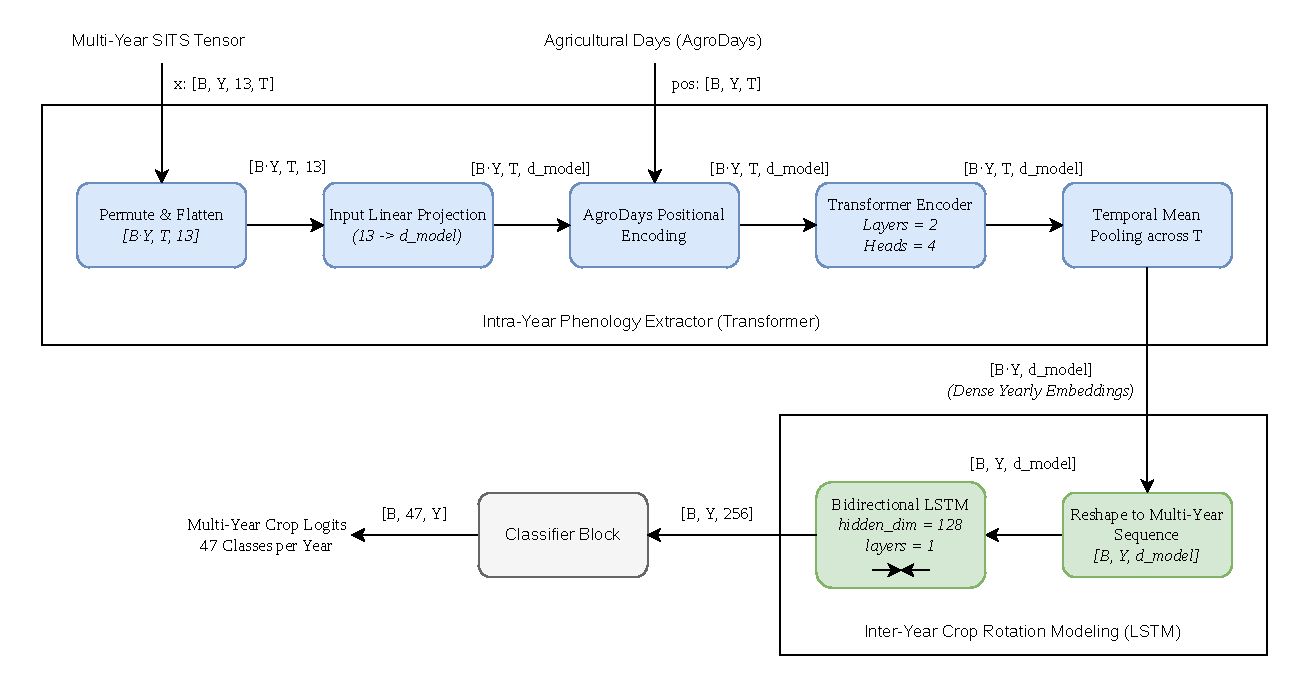
\includegraphics[width=0.9\textwidth]{images/transformer_lstm_diagram.pdf}
    \caption{Hierarchical overview of the Transformer-LSTM architecture, demonstrating the fusion of intra-year and inter-year components.}
    \label{fig:hybrid_architecture}
\end{figure}

\subsection{Capturing Long-Term Crop Rotations}
\label{subsec:crop_rotations}

The primary motivation for integrating the LSTM in the second stage is its exceptional ability to model strict, long-term sequential rules.
Traditional crop mapping architectures primarily focus on extracting phenological features within a single growing season, discarding a vast amount of predictive temporal context.
However, agricultural practices are heavily governed by multi-year crop rotation cycles designed to maintain soil health and comply with policies. 
To explicitly capture these long-term crop rotations, a bidirectional LSTM configuration is employed.
This enables the network to analyze the rotation history in both the forward and backward temporal directions,
effectively predicting a crop based on what was planted in previous years as well as what will be planted in subsequent years.
By analyzing this bi-temporal history, the network learns deep inter-year transition probabilities. 
Finally, the bidirectional output---representing this deeply fused, multi-year context---is passed to a fully-connected classification block.
Because the LSTM is bidirectional, the sequence dimension is explicitly doubled to accommodate the concatenated forward and backward hidden states.
These deep features are passed through a ReLU activation and a dropout regularization layer (set to 10\%) to prevent overfitting.
A final linear projection maps the processed features into the unnormalized logit scores for the 47 target crop classes,
outputting a highly informed prediction for each year in the sequence.


\section{Infrastructure and Optimization}
\label{sec:infrastructure}

Training deep temporal models on massive satellite datasets requires a robust, scalable infrastructure.
To ensure reproducibility, efficient hardware utilization, and systematic hyperparameter selection,
the experimental framework was constructed using PyTorch Lightning \cite{falcon2019pytorch}, Ray Tune \cite{liaw2018tune}, and MLflow \cite{zaharia2018accelerating}.

\subsection{PyTorch Lightning Training Pipeline}
\label{subsec:lightning_pipeline}

The training logic for all models was encapsulated within the PyTorch Lightning framework \cite{falcon2019pytorch},
abstracting code engineering while ensuring multi-GPU scalability.
Several optimizations were implemented at the pipeline level to stabilize training and maximize throughput:

\textbf{Mixed Precision Training:}
To optimize GPU memory and accelerate tensor operations, the trainer was configured to use 16-bit mixed precision (\texttt{16-mixed}).
This allows the models to perform computationally heavy operations in half-precision while maintaining full precision for gradient accumulations,
maximizing the throughput of the underlying hardware.

\textbf{Loss Formulation:}
The networks were trained using a standard Cross-Entropy Loss function.
Crucially, an \texttt{ignore\_index} parameter set to 255 was passed to the loss function.
This ensured that any padded sequences or years dropped during data augmentation did not contribute to the loss gradients or skew the accuracy metrics.

\textbf{Optimization and Regularization:}
Optimization was governed by the AdamW algorithm \cite{loshchilov2017decoupled}.
Unlike the standard Adam optimizer, AdamW correctly decouples weight decay from the adaptive learning rate updates, providing superior regularization \cite{loshchilov2017decoupled}.
To prevent unnecessary computational expenditure on converging models, an Early Stopping callback was implemented,
terminating training if the validation accuracy (\texttt{val\_acc}) failed to improve for 10 consecutive epochs.

\subsection{Distributed Hyperparameter Tuning with Ray Tune and Optuna}
\label{subsec:ray_tune}

Neural network sequence models are highly sensitive to their hyperparameters. To systematically search for the optimal configuration,
a distributed tuning loop was orchestrated using Ray Tune \cite{liaw2018tune},
integrated with the Tree-structured Parzen Estimator (TPE) sampling algorithm from Optuna \cite{akiba2019optuna}.

The tuning process was executed with a budget of 30 total trials.
The Optuna sampler was initialized with 20 completely random startup trials to thoroughly explore the boundaries of the parameter space before
transitioning to a Bayesian optimization strategy. To maximize hardware efficiency, Ray Tune was configured to run 3 trials concurrently.
During this exploratory phase, each trial was trained for a truncated duration of 5 epochs.

\begin{algorithm}[htpb]
    \caption{Distributed Ray Tune and Lightning Orchestration}
    \label{alg:ray_tune}
    \begin{algorithmic}[1]
        \Require Search space $\mathcal{S}$, Trials $N = 30$, Concurrent Workers $W = 3$
        \Ensure Best configuration $config_{best}$ and evaluated Test Metrics
        \vspace{1.5mm}
        \Function{MetaparametersTuning}{$\mathcal{S}$}
            \State $\mathcal{D} \gets \text{Initialize Optuna TPE Sampler}(\text{startup\_trials}=20)$
            \State $results \gets \text{RayTuneRun}($
            \State \quad $\text{train\_fn} = \text{LightningTrainer},$
            \State \quad $\text{search\_space} = \mathcal{S},$
            \State \quad $\text{num\_samples} = N,$
            \State \quad $\text{max\_concurrent} = W,$
            \State \quad $\text{scheduler} = \mathcal{D}$
            \State $)$
            \State $config_{best} \gets \text{GetBestConfig}(results, \text{metric}=\text{'val\_acc'}, \text{mode}=\text{'max'})$
            \State \textbf{return} $config_{best}$
        \EndFunction
        \vspace{1.5mm}
        \State \textbf{Execution:}
        \State $config_{best} \gets \textsc{MetaparametersTuning}(\mathcal{S})$ \Comment{Run 5 epochs per trial}
        \State $Model_{final} \gets \text{InitializeModel}(config_{best})$
        \State $Trainer_{final} \gets \text{LightningTrainer}(\text{max\_epochs}=40, \text{early\_stopping}=10)$
        \State $Trainer_{final}.\text{fit}(Model_{final})$
        \State $TestMetrics \gets Trainer_{final}.\text{test}(Model_{final})$
    \end{algorithmic}
\end{algorithm}

The continuous search space included a log-uniform distribution for the learning rate (bounded between $1\mathrm{e}{-5}$ and $1\mathrm{e}{-2}$) and
the weight decay (bounded between $1\mathrm{e}{-7}$ and $1\mathrm{e}{-3}$). Discrete grid-search choices were provided for the batch size (8, 16, or 32).
Furthermore, architecture-specific parameters were dynamically tuned:
\begin{itemize}
    \item For the \textbf{GRU RNN}, the search space tested hidden dimensions of 128, 256, and 512, alongside variable network depths of 1, 2, or 3 stacked layers.
    \item For the \textbf{Transformer-LSTM}, the core embedding dimension (\texttt{d\_model}) was tested across 128, 256, and 512.
\end{itemize}
Every trial automatically logged its hyperparameters and performance metrics (including training loss, validation loss, overall accuracy, and F1-score)
to a local MLflow database \cite{zaharia2018accelerating}. After the tuning phase concluded, the configuration that yielded the maximum validation accuracy was extracted.
This optimal configuration was then used to instantiate a final model, which was trained from scratch for 40 epochs and rigorously evaluated on the held-out test set.

\begin{table}[htpb]
    \centering
    \renewcommand{\arraystretch}{1.2}
    \begin{tabular}{lll}
        \toprule
        \textbf{Hyperparameter} & \textbf{Distribution/Values} & \textbf{Applies To} \\
        \midrule
        Learning Rate & Log-Uniform $[1\mathrm{e}{-5}, 1\mathrm{e}{-2}]$ & All Models \\
        Weight Decay & Log-Uniform $[1\mathrm{e}{-7}, 1\mathrm{e}{-3}]$ & All Models \\
        Batch Size & $\{8, 16, 32\}$ & All Models \\
        GRU Hidden Dim & $\{128, 256, 512\}$ & GRU RNN \\
        GRU Layers & $\{1, 2, 3\}$ & GRU RNN \\
        Transformer $d\_model$ & $\{128, 256, 512\}$ & Transformer-LSTM \\
        \bottomrule
    \end{tabular}
    \caption{Hyperparameter search space defined for Ray Tune optimization.}
    \label{tab:search_space}
\end{table}